\documentclass[12pt]{article}
\usepackage{fullpage,enumitem,amsmath,amssymb,graphicx}
\usepackage{listings}
\usepackage{tikz}
\usepackage{hyperref}
\usepackage{subfig}
\usepackage{minted}

\begin{document}

\begin{center}
{\Large Introduction to Image Understanding Homework 3}

\begin{tabular}{rl}
Name: &  Anass Belcaid \\
\end{tabular}
\end{center}

By turning in this assignment, I agree by the Stanford honor code and declare
that all of this is my own work.

\section*{Problem 1}

\begin{enumerate}[label=(\alph*)]
  \item \textbf{Feature Extraction}: Write a function to extract  \emph{Sift
      features}.

    \begin{minted}[frame=lines, fontsize=\scriptsize]{python}
      def get_sift_features(Img):
      """
      Wrapper function to get the SIFT features on the image
      """

      if Img.ndim == 3:
      #convert the image to grayscale
      Img = cv2.cvtColor(Img, cv2.COLOR_BGR2GRAY)

      #¢reating the sift instance
      sift = cv2.xfeatures2d.SIFT_create()

      #getting the keypoints
      kp = sift.detect(Img, None)

      return kp


      
      def q1():
      """
      Question 1 compute the SIFT keypoints
      """

      #filenames
      names = ["reference.png", "test.png", "test2.png"]
      sift_names  = ['ref_sift.png', 'test_sift.png', 'test2_sift.png']

      #images
      Imgs = list(map(cv2.imread, names))

      for img, siftname in zip(Imgs, sift_names):
      print("Processing img : {}".format(siftname))
      kp = get_sift_features(img)
      out = img[0].copy()
      cv2.drawKeypoints(img, kp[-100:], outImage = out, flags=cv2.DRAW_MATCHES_FLAGS_DRAW_RICH_KEYPOINTS)
      \end{minted}
    \begin{figure}[ht]
        \centering
      \subfloat[a][reference]{
        
\includegraphics[width=4.8cm, height=4cm]{./ref_sift.png}  
        }
\hfill
        \subfloat[b][test1]{
          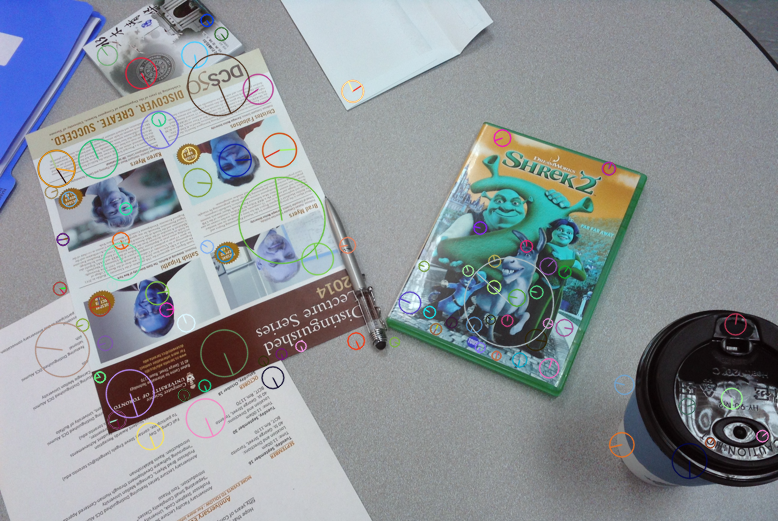
\includegraphics[width=4.8cm, height=4cm]{./test_sift.png}  
        }
\hfill
        \subfloat[c][test2]{
          \includegraphics[width=4.8cm, height=4cm]{./test2_sift.png}  
        }
        \caption{Features Extraction by the SIFT method}
      \end{figure}

    \item Propose a simple \textbf{matching} algorithm:\\

 I will use the simple matching algorithm that compute the \textbf{distances}
 between referenced image and the template. A match is detected is the ratio
 between the \textbf{closest} and next \textbf{closest} is inferior to a given
 constant $C$. Also the matches will be sorted according to distances to their
 associated points.
 \begin{minted}[frame=lines, fontsize=\scriptsize]{python}

def match_descriptors(desc1, desc2, threshold=0.5):
    """
    Match the feature descriptors by finding distances between them. A match is formed 
    when the distance to the closest vector is much smaller than the distance to the 
    second-closest, that is, the ratio of the distances should be smaller
    than the threshold. Return the matches as pairs of vector indices.
    
    Args:
        desc1: an array of shape (M, P) holding descriptors of size P about M keypoints
        desc2: an array of shape (N, P) holding descriptors of size P about N keypoints
        
    Returns:
        matches: an array of shape (Q, 2) where each row holds the indices of one pair 
        of matching descriptors
    """
    matches = []
    
    N = desc1.shape[0]
    dists = cdist(desc1, desc2)

    for i in range(N):
        #getting the indices for the smallest distance
        m1,m2 = np.argsort(dists[i,:])[:2]

        # computing the ratio
        ratio = dists[i,m1]/dists[i,m2]

        #adding the match
        if(ratio<threshold):
            matches.append((i,m1))
     
    return np.array(matches)
 \end{minted}


\begin{figure}[ht]
  \centering
  \subfloat[a][Test1]
  {
    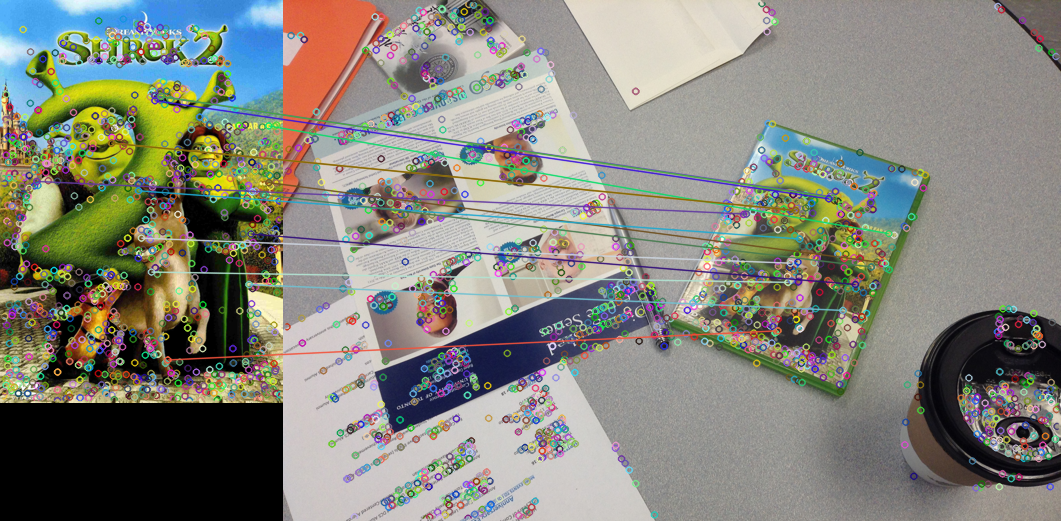
\includegraphics[width=7cm, height=5cm]{./simple_matching1.png}
  }
  \hfill
  \subfloat[b][Test2]
  {

    \includegraphics[width=7cm, height=5cm]{./simple_matching2.png}
  }
  \caption{Matching with distances }
\end{figure}

\item  Find the affine transform  between the  matches

 \begin{minted}[frame=lines, fontsize=\scriptsize]{python}

def find_affine_transform(kp1, kp2, matchs):
    """
    Function to find the affine transform between the set of kp1 and kp2
    """
    
    X = np.array([kp1[i].pt for i in matchs[:3,0]]).T
    #padding X
    X = np.r_[X, np.ones((1,3))]
    Y = np.array([kp1[i].pt for i in matchs[:3,1]]).T
    Y = np.r_[Y, np.ones((1,3))]

    #compute the transofmration matrix
    H = np.linalg.lstsq(X,Y, rcond=None)[0]
    return H

def q3():
    """
    Find affine transformation between template and figure
    """

    template = cv2.imread("./reference.png")
    kp1,desc1 = get_sift_features(template) 

    #reference
    ref = cv2.imread("./test.png")
    kp2, desc2 = get_sift_features(ref)



    #matching desciptors
    matchs = match_descriptors(desc1, desc2)

    #getting the keypoints as (x, y)
    H = find_affine_transform(kp1, kp2, matchs)


    return H
\end{minted}

 \begin{figure}[ht]
   \centering
   \subfloat[a][Test 1]{
     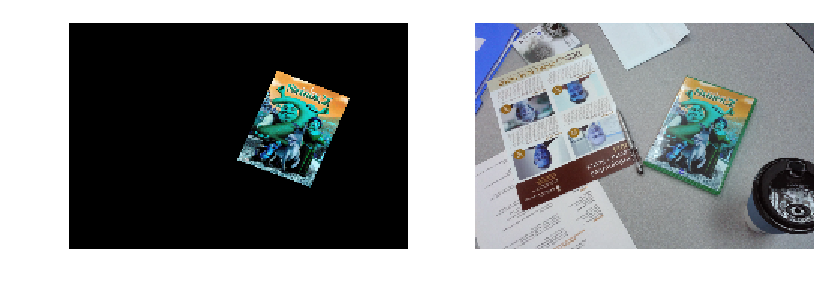
\includegraphics[width=7.5cm, height=8cm]{./linear_transform_test1.pdf}
   }
   \hfill
   \subfloat[b][Test 2]{
     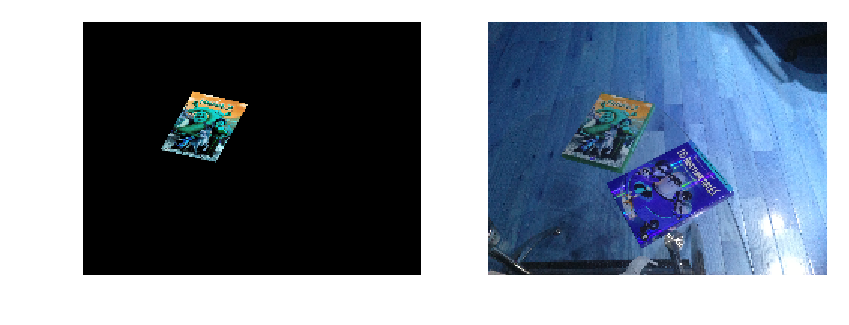
\includegraphics[width=7.5cm, height=8cm]{./linear_transform_test2.pdf}
   }
   \caption{Transformation by the first matches}
 \end{figure}

\end{enumerate}


\end{document}
